\section{Theoretische Grundlagen}
  
  Die High Performance Liquid Chromatography (HPLC) ist ein häufig verwendetes chromatographisches Trennverfahren. Die mobile Phase ist flüssig und durchströmt unter hohem Druck eine Säule, die die stationäre Phase enthält. Aufgrund von unterschiedlich starken Wechselwirkungen der in der mobilen Phase \textit{gelösten} Substanzen mit der stationären Phase kommt es zur Trennung. \citep{SkriptHPLC}\footnote{das ausgegebene Skript referenziert auf \citep{QuantitativeAnalyseHarris}, \citep{InstrumentelleAnalytikSkoog} und \citep{ModernLiquidChromatography} - im Folgenden wird aus Gründen der Einfachheit nur auf das Skript verwiesen}
  
  \subsection{Aufbau der HPLC und Ablauf einer Analyse}
    
    Eine HPLC besteht aus einer Vorrichtung zur Probenaufgabe, einer Vorrichtung zur Lagerung der Lösungsmittel inklusive Entgaser, einer Pumpe, einer Trennsäule, einem Detektor und einem Gerät zur Auswertung. Die einzelnen Bestandteile werden in Abbildung \ref{fig:AufbauHPLC} schematisch dargestellt. Der grundsätzliche Aufbau verändert sich bis auf die Trennsäule und den Detektor nicht. Diese können je nach Analyse ausgetauscht werden. Im Folgenden werden die einzelnen Bestandteile näher beschrieben.
    
      \begin{figure}[H]
        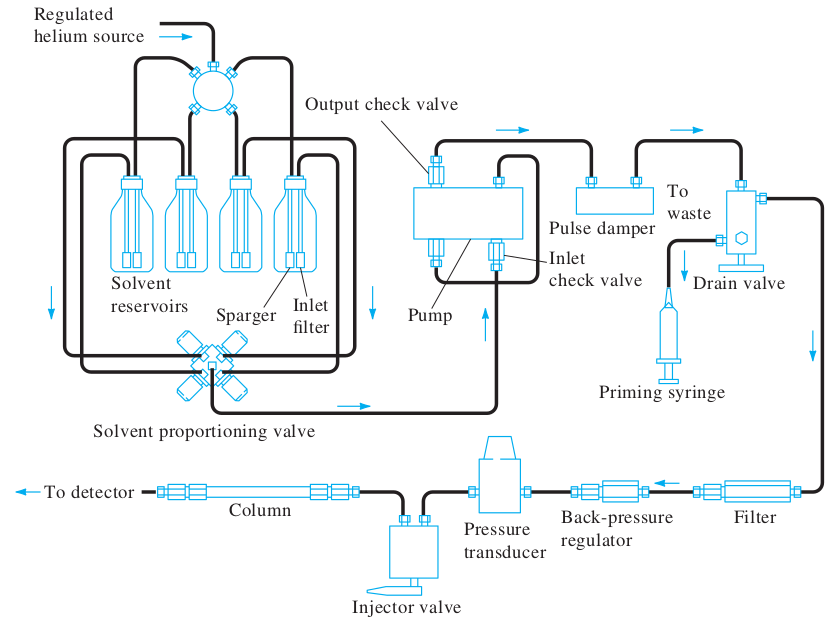
\includegraphics[scale=0.3, center]{images/PartsOfHPLC.png} 
        \caption[Schematischer Aufbau einer HPLC (Eigentum der PerkinElmer Corp., Norwalk, CT), Quelle: \citep{InstrumentelleAnalytikSkoog}]{Schematischer Aufbau einer HPLC (Eigentum der PerkinElmer Corp., Norwalk, CT).}
        \label{fig:AufbauHPLC}
      \end{figure}
      
     \subsubsection{Probenaufgabe}
       
       Die Probenaufgabe erfolgt entweder manuell oder automatisch. Die manuelle Aufgabe wird heutzutage hauptsächlich bei präparativen Trennungen verwendet. Bei der üblichen automatischen Aufgabe erfolgt die Injektion mit einer Spritze über ein 6-Wege Ventil. \citep{SkriptHPLC}
       
         \begin{figure}[H]
           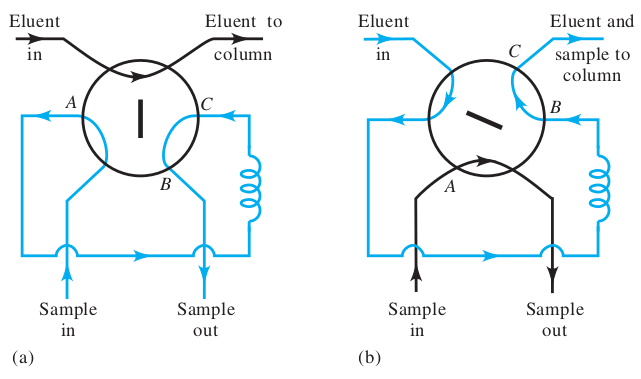
\includegraphics[scale=0.3, center]{images/Funktionsweise6WegeVentil.png} 
           \caption[Beschreibung der Funktionsweise des 6-Wege Ventil, Quelle: \citep{InstrumentelleAnalytikSkoog}]{6-Wege Ventil: in Position (a) wird die Probenschleife ACB gefüllt, in Position (b) wird die Probe mithilfe des Eluenten in die Trennsäule überführt.}
           \label{fig:SechsWegeVentil}
         \end{figure}
         
     \subsubsection{Lösungsmittel und Entgaser}
       
       Häufig wird eine Mischung aus mehreren Lösungsmittel benötigt, um die Polarität der mobilen Phase besser einstellen zu können. Die Zusammensetzung wird über ein Umschaltventil oder durch Verwendung mehrerer Pumpen reguliert - siehe dazu Kapitel \ref{sec:Pumpe}. Der Entgaser entfernt die restlichen Gasteilchen der Laufmittel, da diese die Messung beeinträchtigen können. \citep[S. 749]{InstrumentelleAnalytikSkoog}
       
     \subsubsection{Pumpe und Gradientenentwicklung} \label{sec:Pumpe}
     
       Die Pumpe dient dazu, die mobile Phase unter hohem Druck durch die Trennsäule zu befördern. Man unterscheidet zwischen Hochdruck- und Niederdrucksystemen. Beim Hochdrucksystem wird pro Lösungsmittel eine Pumpe verwendet und durch Einstellung der jeweiligen Flussrate die Laufmittelzusammensetzung bestimmt. In einer Mischkammer werden die Lösungsmittel zum Eluenten vereinigt. Beim Niederdrucksystem reguliert ein Umschaltventil vor der Pumpe die Laufmittelzusammensetzung, wobei bis zu vier unterschiedliche Lösungsmittel gemischt werden. Die Gradientenentwicklung ist im Gegensatz zum Hochdrucksystem schwerfälliger, dafür wird nur eine Pumpe benötigt. \citep{SkriptHPLC}
       
     \subsubsection{Trennsäule}
       
       Die Trennsäule enthält die stationäre Phase. Grundsätzlich unterscheidet man zwischen gepackten und monolithischen Säulen. Sie sollte folgenden Anforderungen genügen: hohe mechanische Festigkeit, chemische Stabilität, homogene Korngröße,
Biokompatibilität, Resistenz gegen Mikroorganismen, keine unspezifischen Wechselwirkungen, hohe Selektivität und konstante Qualität. \citep{SkriptHPLC}

     \subsubsection{Detektor}
     
       Die Wahl des Detektors richtet sich an die physikalischen und chemischen Eigenschaften des Analyten. In Verwendung sind z. B. Brechungsindex-Detektor (RI), Amperometrischer Detektor, Chemischer Reaktionsdetektor, Fluoreszenzdetektor (FLD), Massenspektrometer und Wellenlängendetektor (UV/Vis oder Diodenarray-Detektor, DAD). Im Experiment wird ein DAD verwendet. Dieser kann im Gegensatz zum UV/Vis Detektor die Absorption bei mehreren Wellenlängen gleichzeitig messen und liefert somit zu jedem Zeitpunkt ein vollständiges Chromatogramm. Damit lassen sich unter anderem Rückschlüsse auf Strukturelemente machen. \citep[S. 158]{Taschenatlas}
     
  \subsection{Trennmechanismen und stationäre Phasen}
    
    Durch die unterschiedlich starken Wechselwirkungen der Analyten mit mobiler und stationärer Phase kommt es zu unterschiedlichen Verweilzeiten in der jeweiligen Phase und damit zur Trennung. Die Wahl der stationären Phase bestimmt die Art des Trennmechanismus. Man unterscheidet zwischen Normalphasen-, Umkehrphasen-, Affinitäts-, Ionenaustausch- und Größenausschlusschromatographie. Bei der Normal- und Umkehrphasenchromatographie ist der Wechselwirkungsparameter die Polarität. Sie werden im Folgenden näher beschrieben, da die Umkehrphasenchromatographie im Experiment angewandt wird. 
    
      \subsubsection{Normalphasenchromatographie}
      
        Bei der Normalphasenchromatographie wird eine polare stationäre Phase (z. B. \ch{Al2O3} oder Kieselgel - hydrophile Oberfläche) und eine unpolare mobile Phase (z. B. organische Lösungsmittel wie $n$-Hexan) verwendet. Wird Kieselgel verwendet, sollte keine Base im Laufmittel sein, da diese die Silika-Bindungen aufbricht. Die Retentionszeiten sind proportional zur Stärke der polaren Wechselwirkungen mit der stationären Phase. \citep{SkriptHPLC}
        
      \subsubsection{Umkehrphasenchromatographie}
        
        Bei der Umkehrphasenchromatographie wird eine unpolare stationäre Phase (z. B. Kieselgel derivatisiert mit langen, unpolaren Kohlenwasserstoffketten - hydrophobe Oberfläche) und eine polare mobile Phase (z. B. Gemische von Wasser mit organischen Lösungsmitteln wie Acetonitril) verwendet. Die Retentionszeiten sind proportional zur Stärke der hydrophoben Wechselwirkungen mit der stationären Phase. Die Elutionsreihe beschreibt die Retention in absteigender Reihenfolge: Aliphaten $>$ induzierte und permanente Dipole $>$ Lewis Basen $>$ Lewis Säuren. \citep{Versuchsvorschrift}, \citep[S. 162]{Taschenatlas}
    
  \subsection{Chromatographische Parameter} \label{sec:ChromatographischeParameter}
    
    Um den Trennvorgang sowie die Trennleistung einer Analyse bzw. einer Säule zu charakterisieren, hat sich eine Vielzahl an Kenngrößen und Parametern etabliert, die im Folgenden beschrieben werden.
    
     Um die Position und das Aussehen eines Peaks zu beschreiben eignet sich die Totzeit $t_0$ (Zeit der Probe in der mobilen Phase), die Bruttoretentionszeit $t_B$ (Zeit der Probe in mobiler und stationärer Phase), die Nettoretentionszeit $t_R$ (Zeit der Probe in der stationären Phase - $t_R = t_B - t_0$), die Basispeakbreit $w$ (Anlegen zweier Tangenten in \SI[mode=text]{60}{\percent} Peakhöhe und Bestimmung des Abstandes der Schnittpunkte mit der Basislinie), die Halbwertspeakbreite $w_{1/2}$ (Peakbreite bei halber Höhe) und die Peaksymmetrie $T$ ($T = B / A$ mit Abstand vom Peakanfang zum Peakmaximum $A$ und Peakmaximum zu Peakende $B$ in ca. \SI[mode=text]{10}{\percent} der Peakhöhe). Ist $T$ kleiner als 1, so spricht man von Fronting, ansonsten von Tailing. Im Idealfall liegt der Wert zwischen $0.8$ und $1.2$. 
    
    Wechselwirkungsvorgänge werden durch den Kapazitätsfaktor $k$ (relative Verweildauer des Analyten in stationärer Phase - $k = t_R / t_0$), den Verteilungskoeffizient $K$ ($K = c_S / c_M$ in Analogie zum Massenwirkungsgesetz) und die lineare Strömungsgeschwindigkeit $v$ ($v = L / t_R$ mit Säulenlänge $L$) beschrieben. 
    
    Die Effizienz einer Trennsäule wird durch die theoretische Trennstufenhöhe (Bodenhöhe) $H$ und die Anzahl an theoretischen Böden (Trennstufenzahl) $N$ charakterisiert ($L = N H$). Die Anzahl an theoretischen Böden ist ein Maß für die Anzahl an theoretischen Gleichgewichtseinstellungen des Analyten zwischen mobiler und stationärer Phase und kann mit 
    
      \begin{equation}
        N = 16 \left(\frac{t_R}{w}\right)^2 = 5.54 \left(\frac{t_R}{w_{1/2}}\right)^2
      \end{equation} 
    unabhängig von $H$ und $L$ berechnet werden. Die Bodenhöhe in Abhängigkeit von der linearen Strömungsgeschwindigkeit $v$ wird durch die Van-Deemter Gleichung 
    
      \begin{equation}
        H(v) = A + \frac{B}{v} + C v
      \end{equation}
    beschrieben (Beiträge der Eddy-Diffusion $A$, Longitudinaldiffusion $B$ und des verzögerten Massentransfers $C$). Die Eddy Diffusion beschreibt die unterschiedlichen Wegmöglichkeiten des Analyten in der Säule und ist unabhängig von der Fließgeschwindigkeit. Die Longitudinaldiffusion erfolgt längs zur Säule und nimmt mit steigender $v$ ab. Der verzögerte Massentransfer beschreibt die unvollständige und verzögerte Gleichgewichtseinstellung zwischen stationärer und mobiler Phase aufgrund der bewegten mobilen Phase. Er steigt mit zunehmender Fließgeschwindigkeit. Die maximale Trennleistung erfolgt am Minimum der Kurve - siehe Abb. \ref{fig:VanDeemterGleichung}. 
    
      \begin{figure}[H]
        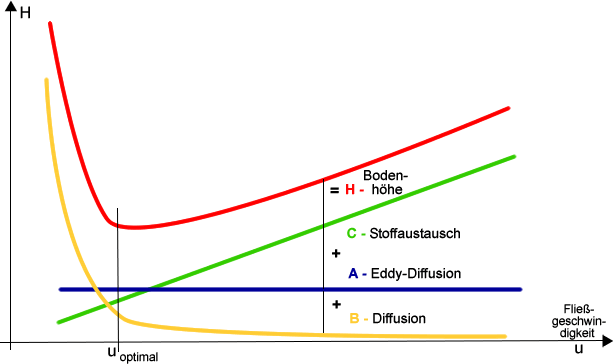
\includegraphics[scale=0.4, center]{images/VanDeemterGleichung.png} 
        \caption[Van-Deemter Gleichung, Quelle: \text{http://www.chemgapedia.de} (Zugegriffen am 07.01.2020)]{Van-Deemter Gleichung mit Illustration der einzelnen Paramter.}
        \label{fig:VanDeemterGleichung}
      \end{figure}    
    
    Die Trennleistung, also die Fähigkeit, zwei benachbarte Peaks eindeutig aufzutrennen, wird durch die Auflösung $R = 2\left(t_{R2} - t_{R1}\right) / \left(w_2 + w_1\right)$ und die relative Retention bzw. Selektivität $\alpha = t_{R2} / t_{R1} = k_2 / k_1$ charakterisiert. Desto größer $R$ und $\alpha$, desto  besser ist die Trennung. \citep{Versuchsvorschrift}
    
  \subsection{Elutionsmechanismen der Umkehrphasenchromatographie}
  
    \subsubsection{Isokratische Elution}
    
      Bei der isokratischen Elution ist die Laufmittelzusammensetzung im Verlauf der gesamten Analyse konstant. Die Methode eignet sich zur Trennung von Molekülen mit ähnlichen Polaritäten.  \citep{SkriptHPLC}
      
    \subsubsection{Gradienten Elution}
      
      Bei der Gradienten Elution wird die Laufmittelzusammensetzung während der Analyse kontinuierlich verändert. Die Methode eignet sich zur Trennung von Molekülen mit stark unterschiedlichen Retentionszeiten bzw. Polaritäten. Anmerkung: das Konzept der in Kapitel \ref{sec:ChromatographischeParameter} vorgestellten theoretischen Böden gilt nur für die isokratische Elution. \citep[S. 156]{Taschenatlas}, \citep{SkriptHPLC}
   
  \subsection{Kalibrierung über einen externen Standard}  
  
    Der verwendete Standard enstpricht dem Analyten, was voraussetzt, dass dieser bekannt ist. Für die Kalibrierung werden mehrere Standardlösungen mit bekannten Konzentration hergestellt und jeweils der Messert bestimmt. In einem Diagramm wird der Messwert auf der Ordinate und die Standardkonzentration auf der Abszisse aufgetragen. Man legt eine lineare Funktion 
    
      \begin{equation}
        y = a + b x \label{eq:externeKalibrierung}
      \end{equation}
    durch die Messpunkte (Fitparameter $a$ und $b$, Messwert $y$ und Konzentration $x$). Anschließend wird die Probe gemessen und man erhält durch Umstellen von \eqref{eq:externeKalibrierung} auf $x$ die Probenkonzentration. Bei der Messung von Standard und Probe müssen die Messbedingungen konstant gehalten werden. Auch sind Matrixeffekt aufgrund unterschiedlicher Zusammensetzungen von Probe und Standard möglich. Dafür benötigt man nur 1 Kalibriergerade für viele Probemessungen. 
  
  %\begin{figure}[H]
    %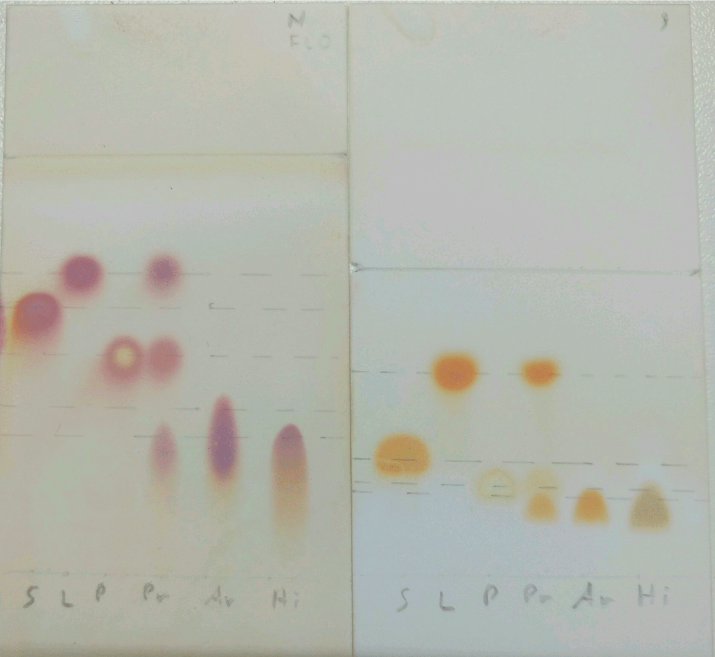
\includegraphics[scale=0.25, center]{images/test.png} 
    %\caption[Quelle: Autor]{Test}
    %\label{fig:Test}
  %\end{figure}
      